\vspace{1em}
\scalebox{0.75}{
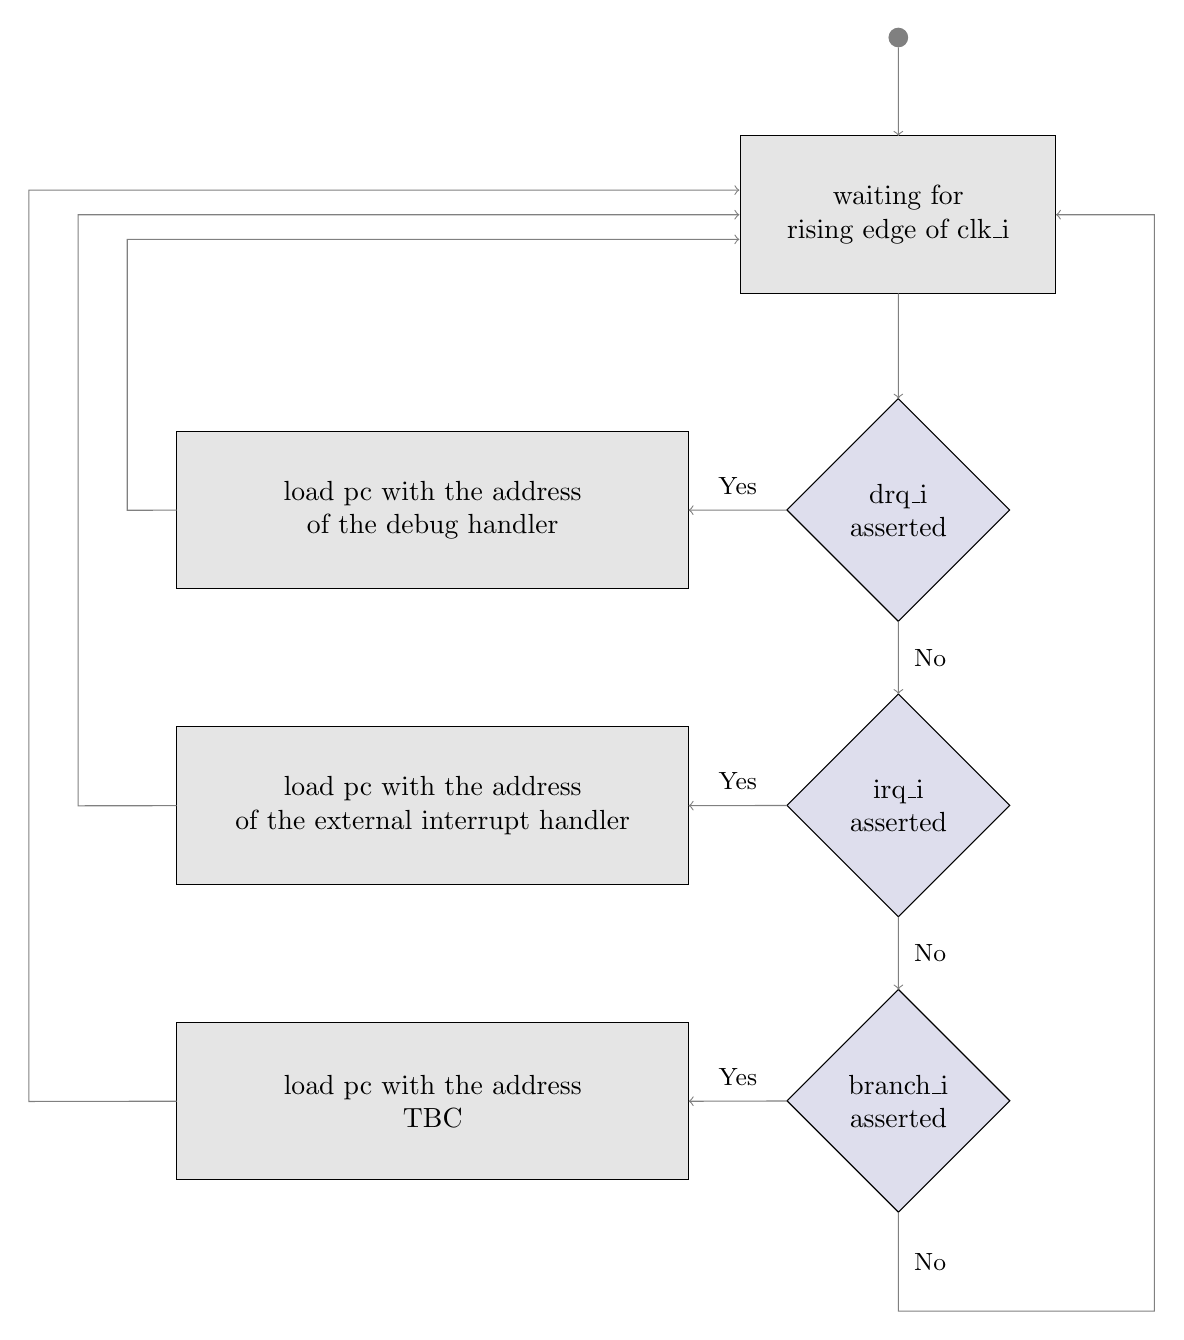
\begin{tikzpicture}[scale=1.25, draw=gray, inner sep=0, outer sep=0]
  \node[rectangle, draw=black,
    align=center,
    anchor=north west,
    minimum height = 2cm,
    minimum width = 4cm,
    fill = gray!20] (box1) at (0, 0) {waiting for\\rising edge of clk\_i};

  \node[rectangle, draw=black,
    minimum height = 2cm,
    minimum width = 2cm,
    rotate=45,
    fill = blue!30!gray!20] (if1) at ([yshift=-3cm]box1.center) {};
  \node[align=center] (if1-text) at (if1.center) {drq\_i\\asserted};

  \node[rectangle, draw=black,
    align=center,
    anchor=east,
    minimum height = 2cm,
    minimum width = 6.5cm,
    fill = gray!20] (box2) at ([xshift=-1cm]if1.north west) {load pc with the address \\ of the debug handler};

  \node[rectangle, draw=black,
    minimum height = 2cm,
    minimum width = 2cm,
    rotate=45,
    fill = blue!30!gray!20] (if2) at ([yshift=-3cm]if1.center) {};
  \node[align=center] (if2-text) at (if2.center) {irq\_i\\asserted};

  \node[rectangle, draw=black,
    align=center,
    anchor=east,
    minimum height = 2cm,
    minimum width = 6.5cm,
    fill = gray!20] (box3) at ([xshift=-1cm]if2.north west) {load pc with the address \\ of the external interrupt handler};

  \node[rectangle, draw=black,
    minimum height = 2cm,
    minimum width = 2cm,
    rotate=45,
    fill = blue!30!gray!20] (if3) at ([yshift=-3cm]if2.center) {};
  \node[align=center] (if3-text) at (if3.center) {branch\_i\\asserted};

  \node[rectangle, draw=black,
    align=center,
    anchor=east,
    minimum height = 2cm,
    minimum width = 6.5cm,
    fill = gray!20] (box4) at ([xshift=-1cm]if3.north west) {load pc with the address \\ TBC};

  \draw[->] (box1.south) -- (if1.north east);
  \draw[->] (if1.south west) -- node[right=0.2cm]{\small No} (if2.north east);
  \draw[->] (if2.south west) -- node[right=0.2cm]{\small No} (if3.north east);

  \draw[->] (if1.north west) -- node[above=0.2cm]{\small Yes} (box2.east);
  \draw[->] (if2.north west) -- node[above=0.2cm]{\small Yes} (box3.east);
  \draw[->] (if3.north west) -- node[above=0.2cm]{\small Yes} (box4.east);

  \node (cross1) at ([yshift=-1cm]if3.south west) {};
  \node (cross2) at ([xshift=1cm]box1.east) {};
  \draw[->] (if3.south west) -- node[right=0.2cm]{\small No} (if3.south west |- cross1.center) -- (cross1.center -| cross2.center) -- (cross2.center) -- (box1.east);

  \node (cross3) at ([xshift=-0.5cm]box2.west) {};
  \node (cross4) at ([xshift=-1cm]box3.west) {};
  \node (cross5) at ([xshift=-1.5cm]box4.west) {};

  \node (cross6) at ([yshift=-0.25cm]box1.west) {};
  \node (cross7) at (box1.west) {};
  \node (cross8) at ([yshift=0.25cm]box1.west) {};

  \draw[->] (box2.west) -- (cross3.center) -- (cross3.center |- cross6.west) -- (cross6.west);
  \draw[->] (box3.west) -- (cross4.center) -- (cross4.center |- cross7.west) -- (cross7.west);
  \draw[->] (box4.west) -- (cross5.center) -- (cross5.center |- cross8.west) -- (cross8.west);

  \node [circle, fill=gray, minimum height = 0.25cm, minimum width = 0.25cm] (start) at ([yshift=1cm]box1.north) {};
  \draw[->] (start.south) -- (box1.north) {};
\end{tikzpicture}
}
